%<dscrpt>Etude d'un système de deux tiges articulées avec des nombres complexes.</dscrpt>
On considère le système plan formé par deux tiges rigides (figure \ref{fig:Eplanicom_1}) de longueur $r_1$ et $r_2$. On suppose $r_2 \leq r_1$ avec $r_2=r_1\sin \Phi$ pour $\Phi \in ]0,\frac{\pi}{2}]$. La première tige tourne autour d'un point fixé, la deuxième tourne autour de l'extrémité de la première.
\begin{figure}
	\centering
	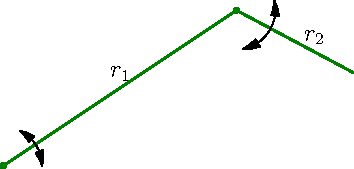
\includegraphics{Eplanicom_1.pdf}
	\caption{Les deux tiges}
	\label{fig:Eplanicom_1}
\end{figure}

On se propose d'étudier quelques questions liées à ce dispositif. En particulier en considérant une relation
\[
z=z_1 + z_2\hspace{0.5cm}
\text{ avec } z=|z|e^{i\theta},z_1=r_1e^{i\theta_1},z_2=r_2e^{i\theta_2}. 
\]
\begin{enumerate}
\item Les figures 2 et 3 présentent deux configurations possibles. En identifiant les points et leurs affixes, placer directement sur les dessins les points $z_1$, $z$, et les angles \emph{orientés} $\theta_1 - \theta$, $\theta_2 - \theta$, $\theta_2 - \theta_1$.
\item On définit les fonctions $f$ et $g$ dans $]0,+\infty[$ par les formules :
\[
f(x)=\frac{x^2+r_1^{2}-r_2^2}{2xr_1},\hspace{0.5cm} g(x)=\frac{x^2-r_1^{2}+r_2^2}{2xr_2}
\]
\begin{enumerate}
\item Former les tableaux de variations de ces fonctions. Préciser les extréma le cas échéant.
\item Préciser : \begin{itemize}
\item l'ensemble des $x$ tels que $f(x)\in [-1,+1]$
\item l'ensemble des $f(x)$ tels que $f(x)\in [-1,+1]$
\item l'ensemble des $x$ tels que $g(x)\in [-1,+1]$
\item l'ensemble des $g(x)$ tels que $g(x)\in [-1,+1]$
\end{itemize}
\item Factoriser $f(x) - g(x)$. En déduire son signe.
\end{enumerate}
\item On suppose $z=z_1 + z_2$ avec $z=|z|e^{i\theta}$, $z_1=r_1e^{i\theta_1}$, $z_2=r_2e^{i\theta_2}$.
\begin{enumerate}
\item Montrer que
\[r_1 - r_2 \leq |z| \leq r_1 +r_2\]
\item Montrer que 
\[
\cos(\theta_1-\theta)=f(|z|), \hspace{0.5cm} \cos(\theta_2-\theta)=g(|z|)\\
\]
\end{enumerate}
\item Soit $z=|z|e^{i\theta}$ avec $r_1 - r_2 \leq |z| \leq r_1 +r_2$.
\begin{enumerate}
\item 
 Montrer qu'il existe un unique couple de réels $(\theta_1,\theta_2)$ tels que
\[
z = r_1e^{i\theta_1} + r_2e^{i\theta_2}  \hspace{0.5cm}
\left\lbrace 
\begin{aligned}
\theta - \theta_1 &\in [0,\Phi] \\
\theta_2 - \theta &\in [0,\pi] 
\end{aligned}
\right. 
\]
Donner des expressions explicites de $\theta_1$ et $\theta_2$ en fonction de $\theta$ et $|z|$.
\item Un tel choix de $(\theta_1,\theta_2)$ conduit-il à une configuration 1 ou 2 ?
\item Montrer que $2\theta \leq \theta_1 +\theta_2$. 
\end{enumerate}

\end{enumerate}
\begin{figure}
	\centering
	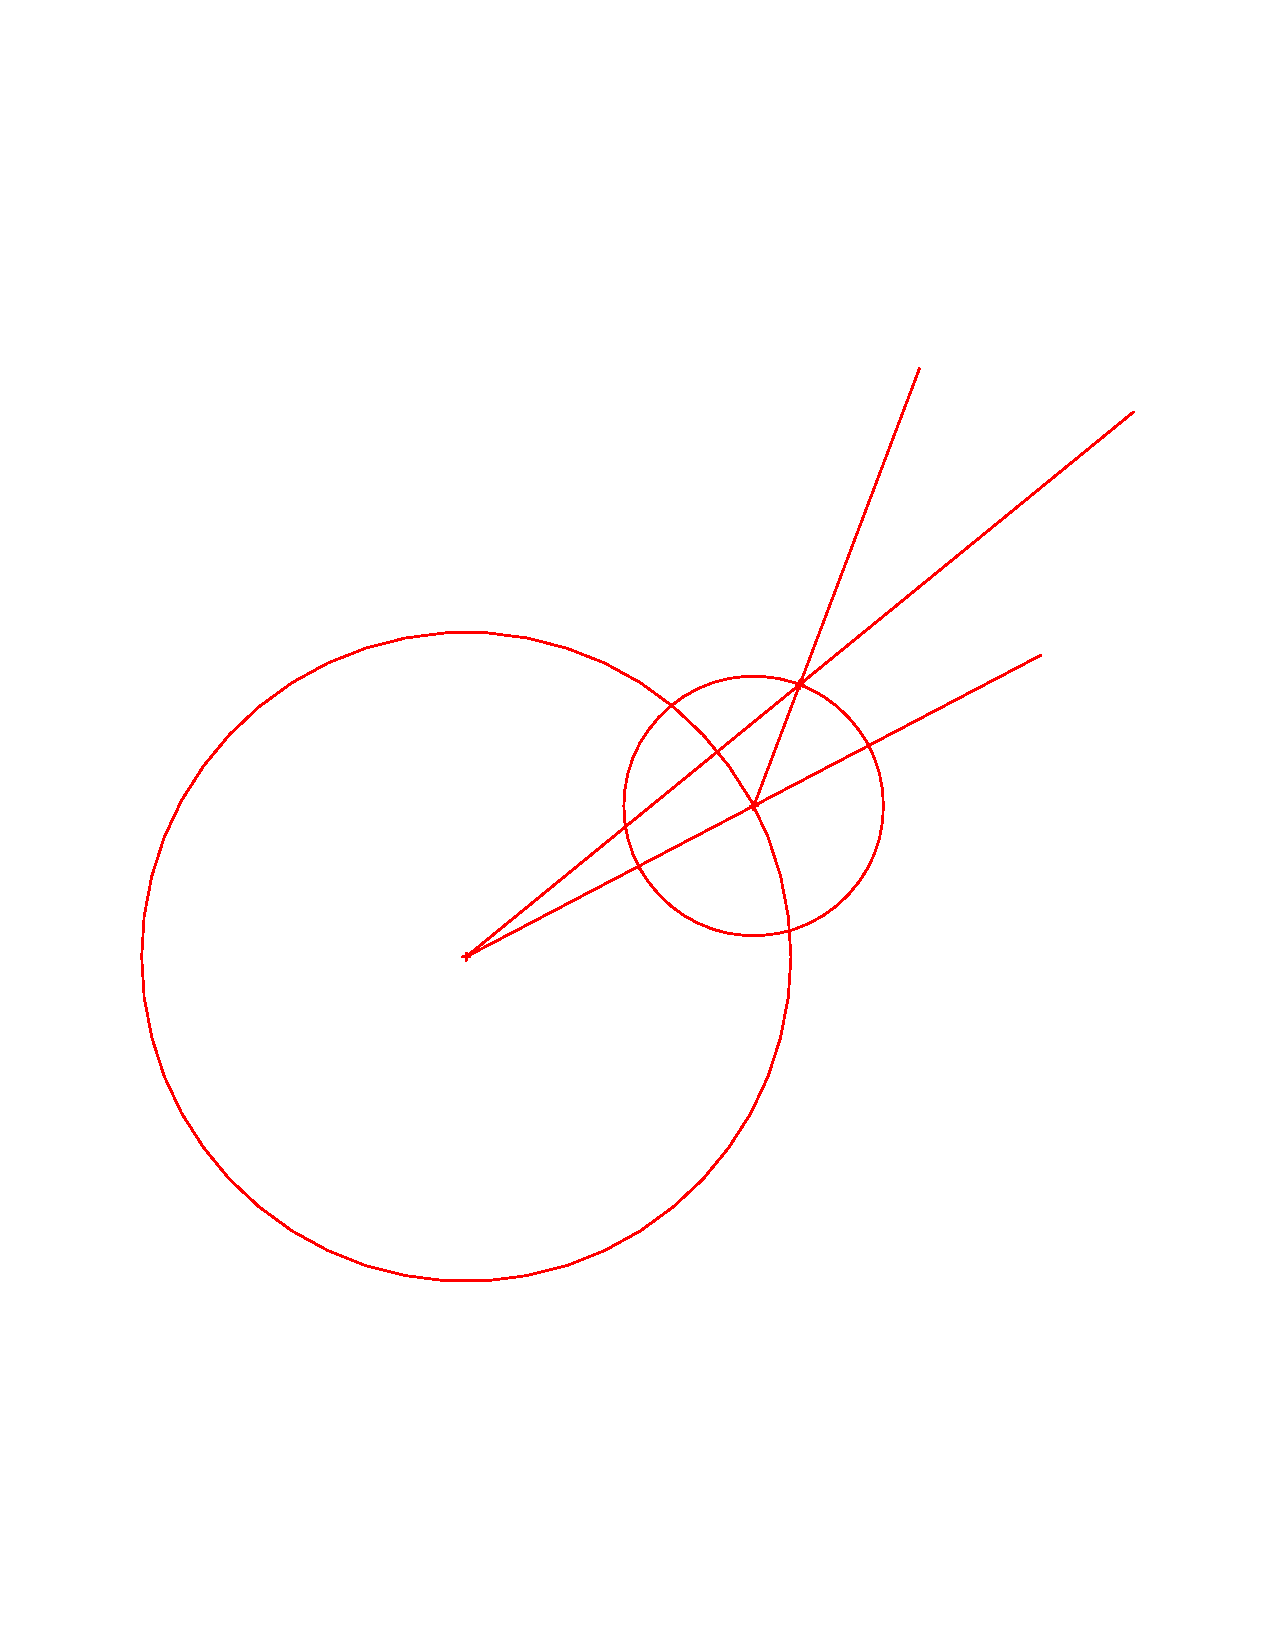
\includegraphics[scale=0.5]{Eplanicom_2.pdf}
	\caption{Configuration 1}
\end{figure}
\begin{figure}
	\centering
	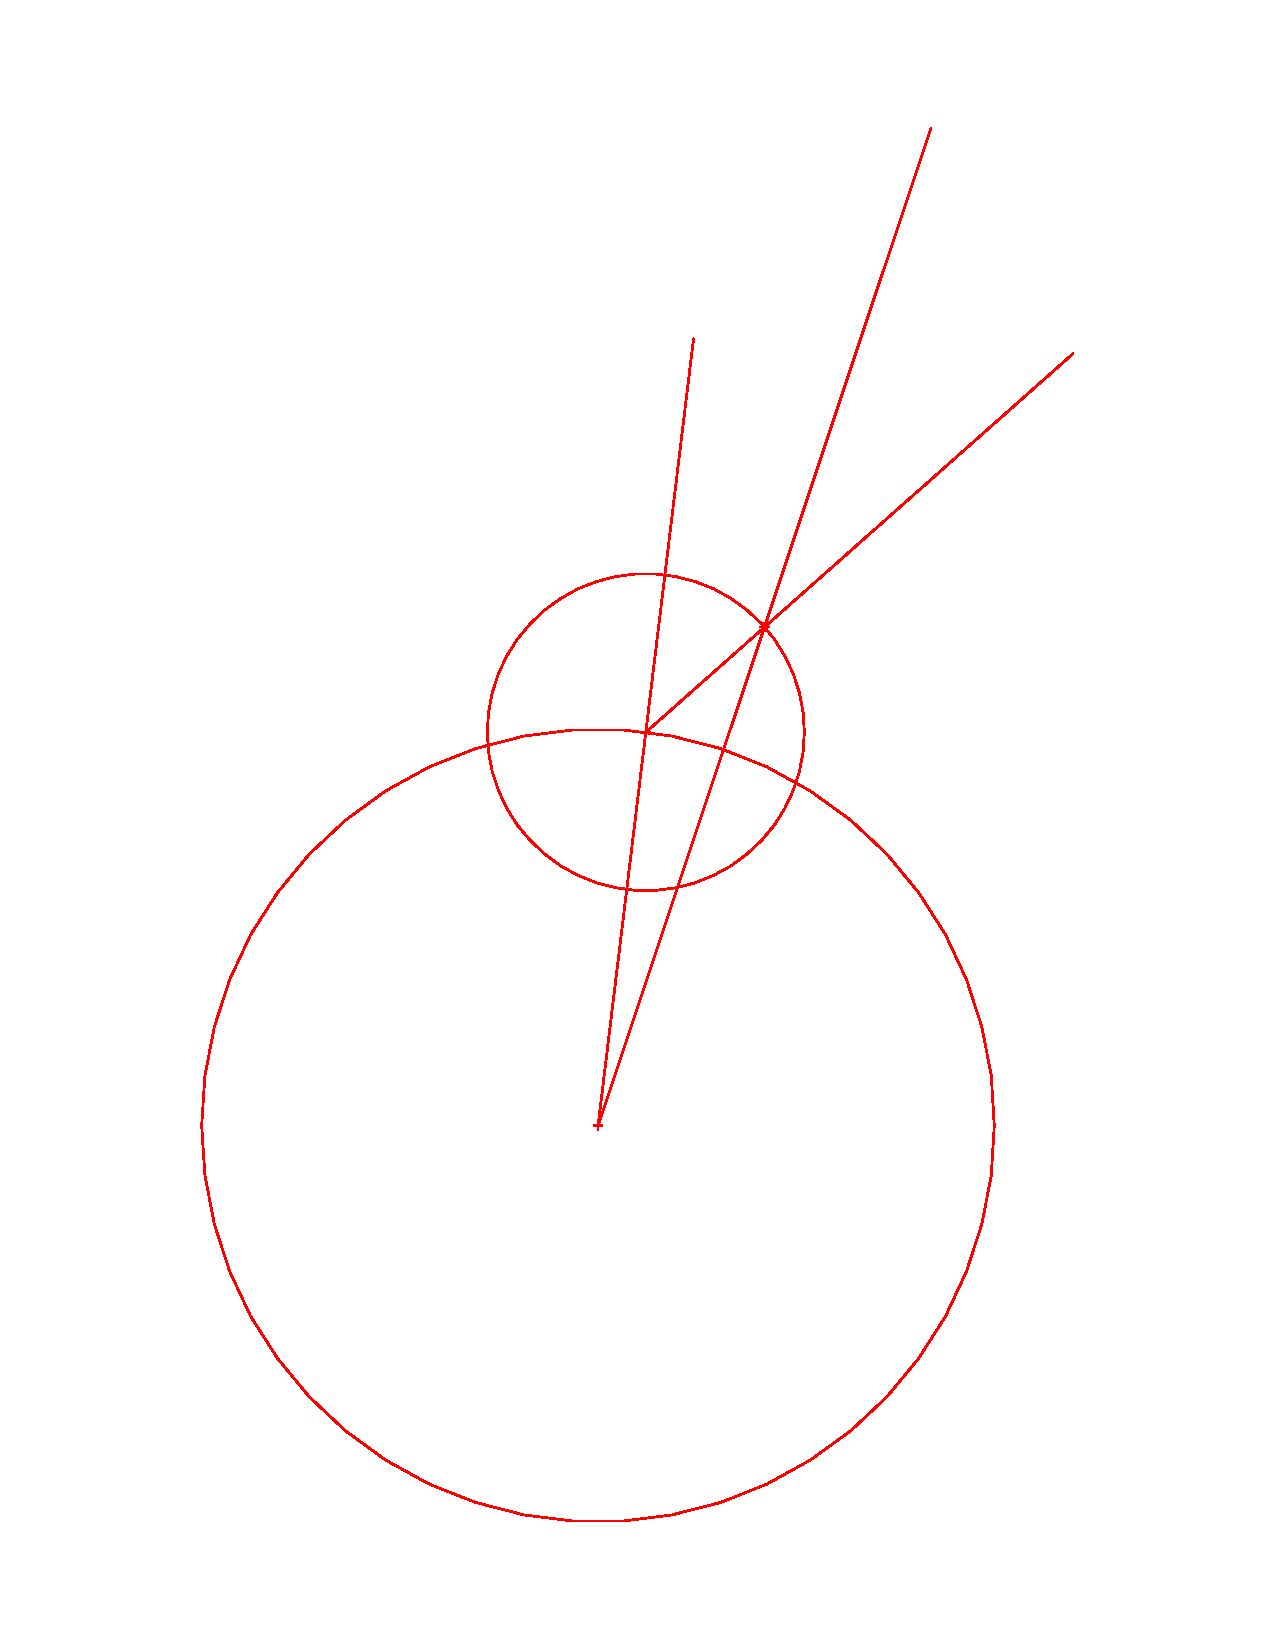
\includegraphics[scale=0.5]{Eplanicom_3.pdf}
	\caption{Configuration 2}
\end{figure}
